\thispagestyle{empty}

\begin{center}
\textsc{\LARGE Aalborg University}\\%[0.5cm]	
\textsc{\Large Geoinformatics}\\[1.cm]
\end{center}

\begin{figure} [H]
	\centering
	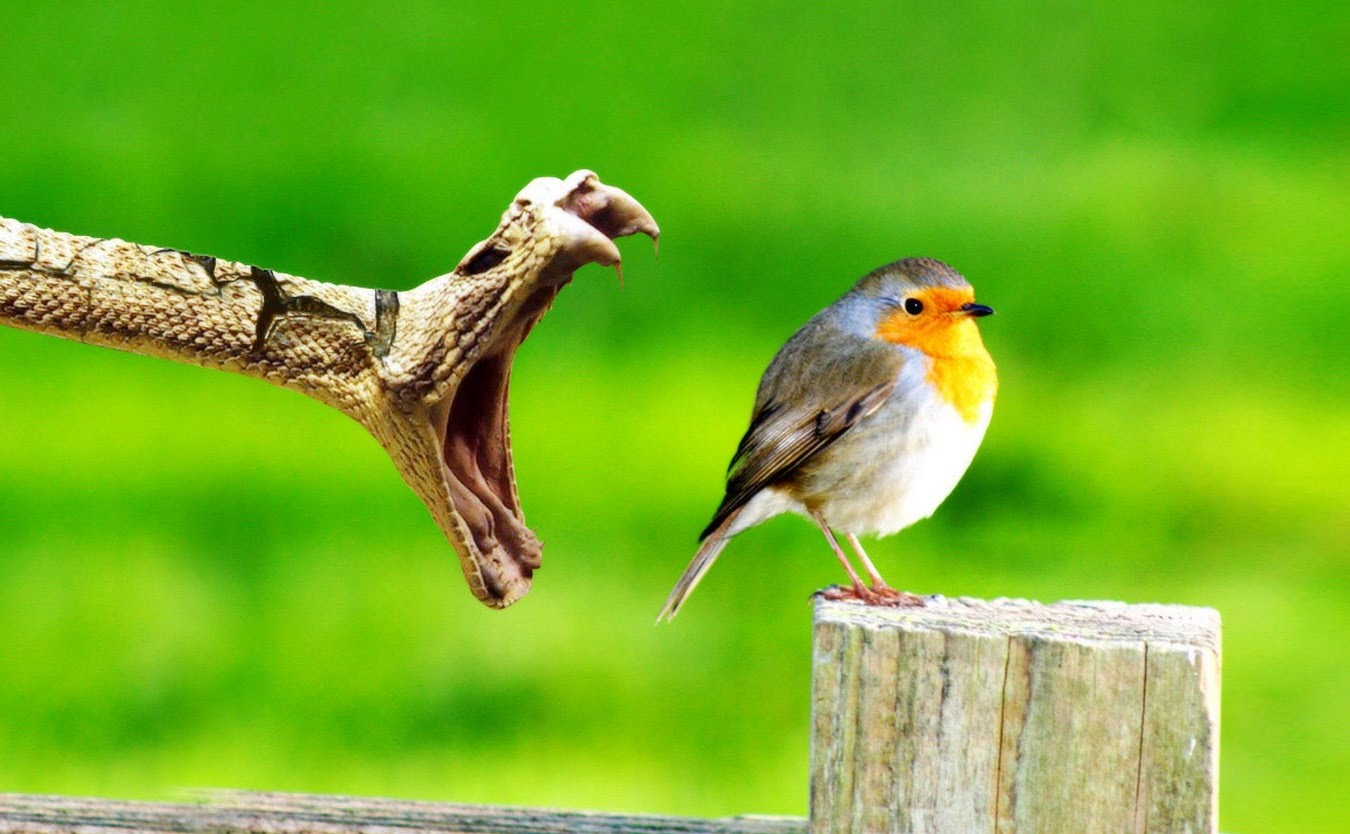
\includegraphics[width=1\textwidth]{Pictures/Example.jpg}	
	\label{forside}
\end{figure}

\vfill
\begin{center}
{ \huge \bfseries {Visualizing and comparing population projection rasters}}\\[0.2cm]
%{\large \bfseries {}}
\end{center}

% Author and supervisor
\begin{tabularx}{\textwidth}{l X r}
	\hline
	\emph{Author:} & & \emph{Supervisors:}\\
	Andreas Gram Riisgaard	&	 &	 Carsten Kessler \\
	\hline
\end{tabularx}

\vfill

% Bottom of the page
{\large January 2019}

\frontmatter

% \begin{figure}[H]
% 	\centering
% 	\includegraphics[width=0.5\textwidth]{billeder/Matrikelkort.jpg}
% 	\caption{Kort over hvilke matrikler, der henholdsvis er under kommunens og skolens ansvar. Udarbejdet af projektgruppen på baggrund af data fra \citep{Skolematrikel}.}
% 	\label{Matrikelkort}
% \end{figure}